    
\chapter{四つ仮名}

\begin{center}
\begin{Large}
第356課: 四つ仮名 
\end{Large}
\end{center}
 
\par{ Yotsugana refers to the four Kana ジ, ヂ, ズ, and ヅ. More strictly speaking, however, it refers to these characters' distinctive pronunciations in Kyoto during the Heian Period. In Modern Japanese, though, how these four are pronounced and used is quite different depending on dialect, and modern spelling changes complicate matters. This lesson will try to take a deeper look into the issue so that you have full control over it. }

\par{\textbf{Curriculum Note }: This lesson uses IPA symbols. }
      
\section{The History of the Pronunciation of ジ, ヂ, ズ, \& ヅ}
 
\par{ In Kyoto (京都) from the late 12th century to the early 14th century, the unvoiced sounds シ, チ, ス, ツ were pronounced as [ɕi] , [ti] , [su] , and [tu] respectively. ɕ is the Japanese sh sound, which is different in articulation than the English sh, and it has been pronounced as such for essentially all of Japanese's written history. However, the pronunciations of チ and ツ have not been so stable. }

\par{ チ and ツ were plosives (sounds that \textbf{stops }all airflow), like the other t-sounds of Japanese, at the time. The voiced equivalents ジ, ヂ, ズ, and ヅ were respectively [ʑi] , [di] , [zu] ,  [du]. Today, the ʑ is the j-sound found inside words. The sounds シ, ジ, ス, and ズ were all fricatives (sounds that force air through a narrow channel). This was audible in Kyoto speech at the time, which is why the distinctions were shown in writing. Had any of these sounds been the same, we would possibly not have some Kana. }

\par{ Problems with this analysis exist. There are words in which \slash z\slash  and \slash d\slash  have been interchangeable since the ancient period. This still happens in dialects today. For instance, some speakers of Japanese pronounce 全然 as "denden". }

\par{ Examples of interchangeability in 四つ仮名 can be found in the word for whale.  クジラ and クヂラ can both be found in the Kanchi'in Ruijumeigishō (観智院本『類聚名義抄』) Dictionary of 1251.  Also during this time, people in the Kanto Region of Japan were mixing [zu] and [du] and [ji] and [di] in many words. It is believed that the spread of making these four sounds into two pairs of homophonous sounds started there. And, in the Tohoku Region, all four became homophonous to dzɯ̈. }

\par{ From the early 14th century to the late 16th century, チ, ツ, ヂ, and ヅ became affricated (starting as a stop but releasing as a fricative). This made them [ʑi] ,[zu] , [ʥi] , and [ʣu] respectively, causing the differences between them narrower. From then on, people would mix up ジand ヂ and ズ and ヅ. So, although 水 was traditionally spelled as  みづ, みず became more common. Likewise, 本寺 is supposed to be ほんじ, but ほんぢ was also used. By the end of the 16th century in places like Niigata, pronunciations had already shifted to the Modern Tokyo pronunciations. However, in places like Kyushu far removed from where these sound changes were taking place, the traditional distinctions were maintained. }

\par{ From the 17th century to the late 19th century, this trend continued to spread. By the end of the 17th century, ヂ \slash ʥi\slash  became ジ [ʑi] and ヅ \slash ʣu\slash  became ズ [zu] even in Kyoto. However, the current conditional sound changes seen in Modern Tokyo speech started to develop. The affricate pronunciations returned before ん. And, depending on dialect, the affricate pronunciations were used in the word initial position. So, words that traditionally started with [ʑi] were regularly being pronounced with [ʥi] instead. }

\par{ Certainly by the end of the 17th century, the pronunciations in Tokyo had already become what they are today. So, today ジ = [ʑi], ヂ [ʥi] =, ズ = [zɯ],  and ヅ = [dzɯ]. ɯ represents the Standard Japanese pronunciation of う, and [u], which is like the English u, is found in other dialects of Japanese. This will be reflected in the transcriptions throughout this lesson. So, take note of these small details. }

\par{\textbf{Regional Note }: Much of this history is centered around Kyoto. Remember that 四つ仮名 started to be confused in other parts of Japan far more quickly. These regions eventually influenced Kyoto speech to bring about the changes mentioned in this discussion. Once the current changes had developed in Niigata and Kyoto, they would then be transplanted into what would become 標準語. Later in this lesson, we will see the paths other dialects took. }
      
\section{Spelling Problems}
 
\par{ How these sounds should be written is not easy because of dialectical variation. The first book to standardize 四つ仮名 spellings was the 1695 ${\overset{\textnormal{けん}}{\text{蜆}}}$ ${\overset{\textnormal{しゅく}}{\text{縮}}}$ ${\overset{\textnormal{りょう}}{\text{涼}}}$ ${\overset{\textnormal{こ}}{\text{鼓}}}$ ${\overset{\textnormal{しゅう}}{\text{集}}}$ . The first four characters when read with their native readings are examples of 四つ仮名. 蜆 = 蜆 (kind of clam), 縮み = ちぢみ (shrinkage), 涼み = すずみ (cooling off), and 鼓 = つづみ (hand drum). It proposed maintaining spelling differences, though only the elite and educated would care. What can be seen in the examples, however, is the still standing rule of when a sound is doubled but voiced, you use the 四つ仮名 variant for that sound. So, although 縮み is pronounced as チジミ, you still write it as チヂミ. Why? Well, that's the big question. }

\par{ Fine, influential people want to maintain a system they've learned and propagated. However, it turns out that even literary geniuses such as 松尾芭蕉 didn't always spell things to standard. You can find him spelling 出づ, the classical form of 出る, as 出ず. }

\par{1. ついに ${\overset{\textnormal{みち}}{\text{路}}}$ ふみたがえて石の巻といふ ${\overset{\textnormal{みなと}}{\text{湊}}}$ に出ず。 \hfill\break
We ended up going the wrong way and entered a harbor called Ishinomaki. }
\textbf{}
\par{ In the Meiji Period, traditional orthography was maintained, but with the turn of the 20th century, 四つ仮名 spelling simplified to じ and ず respectfully, only allowing ぢ and づ used for 連濁  and agreement such as in つづく. However, you can find examples like つまづく (to stumble) being spelled as つまずく, ignoring etymological voicing altogether. }

\par{ So, should students lose points for writing out 鼻血 as はなじ? I would because it's standardized as such, but does that mean the current system shouldn't be altered? There are two paths that could be taken to resolve the problem. }

\par{1. Align spellings to Modern Japanese pronunciation. \hfill\break
2. Revert back to the traditional spellings of 四つ仮名. }

\par{ Either way, the spellings of many words would be changed, but they would be changed to spellings that have been used in the past and in some cases are still being used. Why should we care, though? Only those that like script reform and debates over orthography would probably care, but it's important to know as 四つ仮名 allows us to study Japanese pronunciation in more detail. }
      
\section{Modern Handling of 四つ仮名}
 
\par{ Though the exact pronunciation of 四つ仮名 fluctuates among Tokyo speakers, updates to the government's standard on this have been made as recently as 1986. Though the government's suggestions have no legal bearing on people, traditional distinctions such as 葛 (vine) being くず and 屑 (trash) being くづ have become abandoned. The same goes for 富士 (Fuji) and 藤 (wisteria), which were ふじ and ふぢ respectively. }

\par{ Even so, we still have はなぢ, おこづかい (allowance), きづく (to notice), and つづく as exceptions, though the reason for why they are spelled that way is systematic and based on etymology. At one point, you could write a doubled voiced sound with ゞ (this character is an example of an 踊り字), but sadly this easy fix to the problem has not been used frequently since the end of the war. You still see it in the company name いすゞ, however. This spelling also happens to be easily accessible when typing. }

\par{ So, what about cases such as つまづく・つまずく? つまづく is a clear combination of 爪 (nail) and the suffix -付く, but in the minds of speakers, the compound origin of this phrase has been lost to the point that both spellings are common. This may seem like a wishy-washy standard, but it is exactly how people decide whether both spellings are allowed for etymologically compound words in which ぢ and づ are produced. }

\par{ However, what has caused great debate is the blatant ignoring of obvious compounding and using じ and ず anyway. The most egregious example is spelling the suffix ~中 as じゅう instead of ぢゅう. Another bad example is 稲妻 (lightning), clearly made of いな+ づま, being spelled as いなずま. }

\begin{center}
 \textbf{In Names }
\end{center}

\par{ As you can imagine, if names can be read in so many different ways and spelled in so many different ways in 漢字, 四つ仮名 in names is rather random. For example, 千津子 is typically read as ちづこ, but some people read it as ちずこ. There isn't any pronunciation difference, and both readings can be used to type the name. }

\begin{center}
 \textbf{Changing the Spellings of the Readings of 漢字 }
\end{center}

\par{ Though to a degree, this is what's going on above, the most fundamental changes to Japanese script in regards to 四つ仮名 has been the fundamental altering of spellings to じ and ず that were historically  ぢ or づ since being acquired from Chinese. For instance, 地 had the readings チ and ヂ, being acquired at different times. So, words like 地震 came into Japanese as ヂシン, not ジシン. Furthermore, the word is still pronounced as ヂシン. See the problem?  The reason for changing the spelling is that the reading ヂ came in as such  and was not a change due to 連濁. }

\begin{center}
 \textbf{Reality and the Ignoring of Dialectical Pronunciations }
\end{center}

\par{ Of course, 地 is not the only example. 頭痛 should be づつう and 直に should be ぢきに, but that is just not how they're spelled anymore. This is despite the fact that there are still areas of Japan where 四つ仮名 distinctions are maintained. Even when writing out the dialects of these regions, it is not policy to distinguish them correctly in writing in favor of the standardized spellings. }

\begin{figure}[h]
\centering

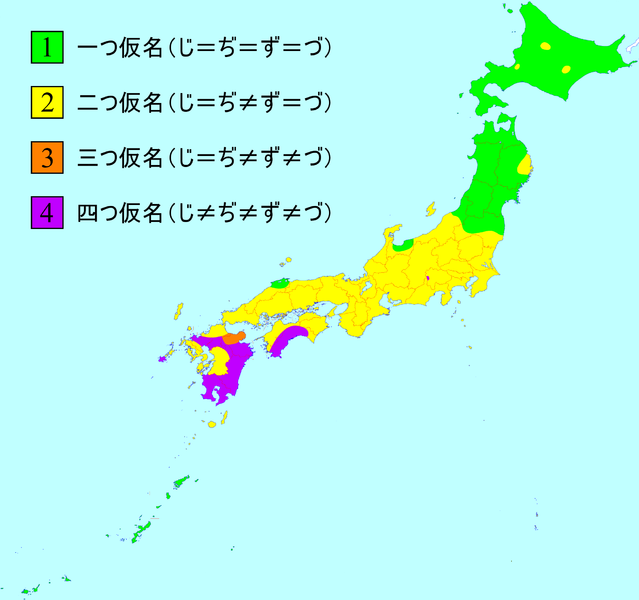
\includegraphics[width=0.9\textwidth]{figs/第08章/第356課:_yotsugana_fig/639px_Yotsugana.png}

\end{figure}
\hfill\break
\textbf{Picture Notes }: 1. This is a distribution based on the speech of older speakers. Many regions marked as other colors have been progressively changing to 二つ仮名弁. It is to note, though, that 一つ仮名弁 still hold strong to various degrees in Tohoku and Izumo. Izumo is the other part of green in the Chuugoku Region (中国地方) to the west of the Kinki Region (近畿地方).  2.The map does a poor job giving clarity to Okinawa, where several other Japanese languages have developed over the centuries. They should not be confused with this phenomenon as other major sound inventory changes have occurred in them, and as you can expect, these changes are not the same. It's just as bad to assume that those sound changes would be the same as thinking the sound changes in English and German have been the same over time.  \textbf{Example Words }  A lot has been said about what 四つ仮名. You've seen examples of words that have had their spellings changed and why, and you should have a sense as to why some things may have alternative spellings. The chart below will try to compile this information together with many examples so that the facts discussed so far become more concrete.  
\begin{ltabulary}{|P|P|P|P|P|P|P|P|}
\hline 

Word & Spell Change? & Original & New & Word & Spell Change? & Original & New \\ \cline{1-8}

泉 & Yes & いづみ & いずみ & 案じる & No & 案じる & 案じる \\ \cline{1-8}

味 & Yes & あぢ & あじ & 言伝て & No & ことづて & ことづて \\ \cline{1-8}

雫 & Yes & しづく & しずく & 埋める & Yes & うづめる & うずめる \\ \cline{1-8}

傷 & No & きず & きず & 築く & Yes & きづく & きずく \\ \cline{1-8}

それじゃ & Yes & それぢゃ & それじゃ & ずつ & Yes & づつ & ずつ \\ \cline{1-8}

ネズミ & No & ネズミ & ネズミ & 恥 & Yes & はぢ & はじ \\ \cline{1-8}

短い & No & みじかい & みじかい & 譲る & Yes & ゆづる & ゆずる \\ \cline{1-8}

水 & Yes & みづ & みず & 羊 & No & ひつじ & ひつじ \\ \cline{1-8}

虹 & No & にじ & にじ & つづら & No & つづら & つづら* \\ \cline{1-8}

沈む & Yes & しづむ & しずむ & 頷く & Yes\slash No & うなづく & うなづく・うなずく \\ \cline{1-8}

\end{ltabulary}
 *: つづら (wig) may be shortened to づら, making it one of the only examples where づ is allowed at the beginning of a word. Another similar example is 痔 (hemorrhoids), which although is historically and currently spelled as じ, and can be written as ぢ in emphatic instances.  \textbf{Reverting Back? }  Because [ʑi] and [ʥi] are allophones (variants using in specific environments) of the same sound and [zɯ]  and [dzɯ] are allophones of the same sound in Standard Japanese, these speakers still technically could re-institute previous pronunciations of words to go back to how 四つ仮名 was used. In singing, there is a tendency to affricate ぢ and づ, but aside from this, most speakers are generally unaware that there are seemingly two set of pronunciations in 四つ仮名: the fricative and the affricate pronunciations.   Most people will think 頭痛 as ずつう despite the fact that they probably pronounce it as づつう. People don't tend to notice these things if they aren't contrasting elements. Because these pronunciations no longer contrast words anymore, it's hard for speakers to even notice the definition, much less intentionally re-institute them into words they were once in.    The idea is nice at its surface, but the problem is that those that support re-instituting proper distinctions in pronunciation in 四つ仮名 typically don't know much about linguistics. Nor do they typically accurate describe the actually phonological processes going on. Many are unaware that words used to begin with ヂ and ヅ, and they sounded differently than words that begin with  ジ and ズ.   It's also not the case that there aren't any examples of ジ and ズ becoming  ヂ and ヅ. After all, we have seen already all words beginning in ジ and ズ be pronounced initially with ヂ and ヅ instead in Standard Japanese. And, again, in the day when spelling wasn't standardized, in areas that 四つ仮名 were being heavily confused with each other, you could see words like 鯨 spelled as  くじら or くぢら. This suggests not just interchangeability in writing but interchangeability in pronunciation.  \textbf{Typing Issues }   Another problem is typing. To type ぢ and づ, you usually type di and du respectively. When Japanese speakers go from Romaji to Japanese input, they often mess up just like foreigners and type in ji and zu respectively, only to find out that the spelling doesn't show up. As time goes on, however, future IME systems may simply 四つ仮名 input to go along with any potential further simplification of them.       
\section{四つ仮名 in Dialects}
 
\par{ As has been discussed thus far, 四つ仮名 have been and continue to be pronounced differently in different dialects. As the picture above demonstrates, a dialect could fall under one of four categories in respect to 四つ仮名. }

\par{一つ仮名弁: Dialects in which じ = ぢ=ず=づ \hfill\break
二つ仮名弁: Dialects in which じ = ぢ≠ ず=づ \hfill\break
三つ仮名弁: Dialects in which じ = ぢ≠ ず≠ づ \hfill\break
四つ仮名弁: Dialects in which じ ≠ ぢ ≠ ず ≠ づ }

\par{ 標準語 is a 二つ仮名弁, just in case you didn't know. However, as we've seen, there are certain environments that allow for all four distinct pronunciations to be used. This categorization tells not how exactly they are pronounced but how they are used contrastively. In 四つ仮名弁, these sounds are all used to contrast words. So, the main focus in this section will be to study how exactly 四つ仮名 are pronounced in various dialects of Japanese. }

\begin{center}
 \textbf{一つ仮名弁 }
\end{center}

\par{ In 一つ仮名弁, there are two ways of saying them all based on specific dialect. If you are a speaker of Kita-ou'u Dialect (far north in Tohoku) or Unpaku Dialect (in Izumo), you pronounce them all as [ʣï]. The vowel is in between い and う as the two vowels merged in this region.  If you are a speaker of Minami-ou'u Dialect, you pronounce them all as [ʣɯ̈]. Because of this, these dialects have been given the stereotypical name ズーズー弁. }

\begin{center}
 \textbf{四つ仮名弁 }
\end{center}

\par{ The completely opposite of 一つ仮名弁 are 四つ仮名弁. However, even though a dialect may have all four as separate sounds, these separate sounds are not uniformly the same throughout these dialects. Many parts of Kyushu, Kouchi Prefecture (高知県), the south of Nara Prefecture (奈良県南部), and Narada in Yamanashi Prefecture (山梨県奈良田) are all areas with 四つ仮名弁. }

\par{ In 高知県, dialects may have the following pronunciations: ジ = [ʑi], ズ = [zu], ヂ = [di] ~ [d z i], ヅ= [du] ~ [d z u]. In Kagoshima Dialect (鹿児島弁),  ジ =[ʑi], ズ = [zu], ヂ = [ʥi], and ヅ = [ʣu]. }

\begin{center}
 \textbf{The Oddity of Narada Dialect in Yamanashi Prefecture }
\end{center}

\par{ Narada is strength with its unique pronunciations: ジ = [ði], ズ = [ðu\slash dzu\slash zu], ヂ = [ɖʐi], ヅ = [ɖu\slash du]. It is also important to note that ツ = [tu] in this dialect. The ð is in English words like "that". These speakers would at least have less difficulty in one sound in English than other Japanese speakers. However, these speakers are dwindling very quickly as many are converting their speech to 標準語 standards. }

\par{ Narata Dialect is first transitioning into a 三つ仮名弁  with most speakers not distinguishing じ and ぢ, though they may still not be exactly like in Standard Japanese. For the most part,  the pronunciation reflects traditional orthography, but there are some words in Narada Dialect in which the sounds have flipped. So, for instance 葛 = 屑 as くず. Although 渦 was うづ, it is rendered as うず, which means it is either pronounced as [uzu], [udzu], or [uðu].  }

\par{\textbf{Research Note }: To hear sound files of Narada Dialect for this information, see http:\slash \slash home.hiroshima-u.ac.jp\slash ikonishi\slash narada\slash narada\_ tu\&du.html  . }

\begin{center}
 \textbf{三つ仮名弁 }
\end{center}

\par{ 三つ仮名弁 are not that common, but some speakers may naturally pronounce 四つ仮名 in this way at times regardless of dialect. Anyway, in these dialects such as 大分弁, ジ = ヂ, butズ doesn't sound like ヅ, which are [zu] and [dzu] respectively. }

\begin{center}
 \textbf{二つ仮名弁 }
\end{center}

\par{ As was said before, there is variation even among 二つ仮名弁. In 京都弁 where the allophonous (varying in specific environments) pronunciation rules developed, most speakers now lightly affricate all these sounds except AFTER ん. In recent years due to the contact of peoples from different parts of the country, and because script reform has gotten rid of the need to notice any traditional differences in pronunciation, most dialects are becoming 二つ仮名弁. }

\par{\textbf{Transcription Note }: Symbols in IPA (International Phonetic Alphabet) are used in this lesson to make transcription as accurate and easy as possible. To look up glyphs that you don't understand, simply copy and paste the problematic ones into Wikipedia where you can find audio tapes for them. }
    